\documentclass{standalone}
\usepackage{tikz}
\usepackage{verbatim}
\begin{document}
\pagestyle{empty}
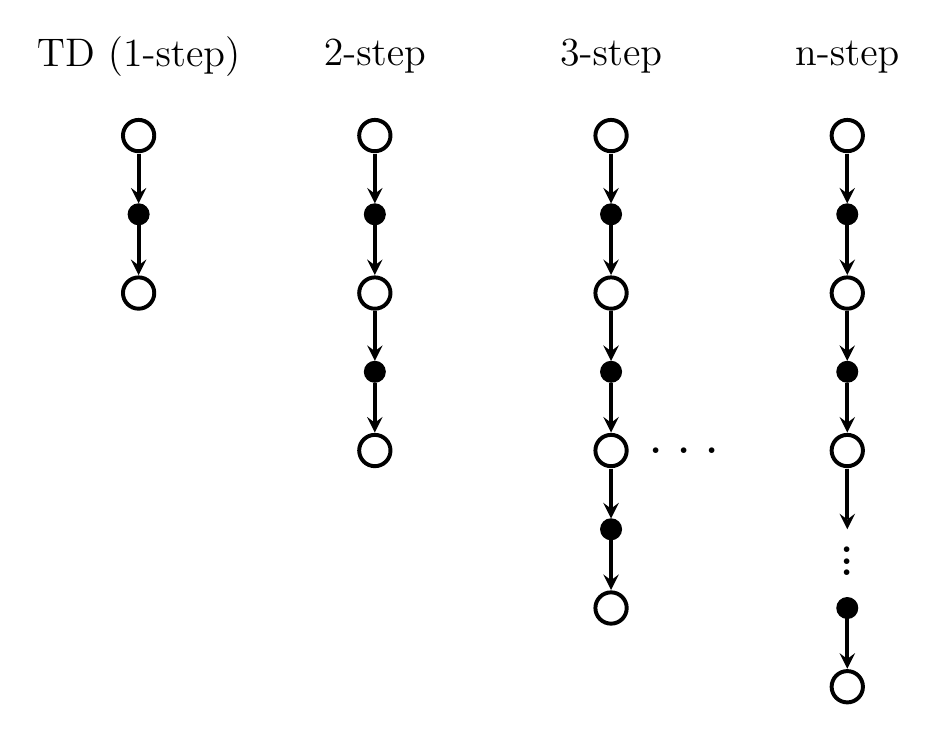
\begin{tikzpicture}


  % TD 1 step
  \node at (0, 1) {\Large TD (1-step)};
  \node[draw,circle,scale=1.2, fill=white, line width=0.5mm] (s_0) at (0,0) {};
  \foreach \xa in {-1} {
      \node[draw,circle,fill,scale=0.8] (b0\xa) at (0, \xa) {};
      \node[draw,circle,scale=1.2, fill=white,line width=0.5mm] (s0\xa) at (0,\xa-1) {};
      \draw[-stealth, line width=0.5mm] (b0\xa) -- (s0\xa);
  }
  \draw[-stealth, line width=0.5mm] (s_0) -- (b0-1);
  
  % TD 2 step
  \node at (3, 1) {\Large 2-step};
  \node[draw,circle,scale=1.2, fill=white, line width=0.5mm] (s_3) at (3,0) {};
  \foreach \xa in {-1,-3} {
      \node[draw,circle,fill,scale=0.8] (b3\xa) at (3, \xa) {};
      \node[draw,circle,scale=1.2, fill=white,line width=0.5mm] (s3\xa) at (3,\xa-1) {};
      \draw[-stealth, line width=0.5mm] (b3\xa) -- (s3\xa);
  }
  \draw[-stealth, line width=0.5mm] (s_3) -- (b3-1);
  \draw[-stealth, line width=0.5mm] (s3-1) -- (b3-3);
  
    % TD 3 step
  \node at (6, 1) {\Large 3-step};
  \node[draw,circle,scale=1.2, fill=white, line width=0.5mm] (s_6) at (6,0) {};
  \foreach \xa in {-1,-3,-5} {
      \node[draw,circle,fill,scale=0.8] (b6\xa) at (6, \xa) {};
      \node[draw,circle,scale=1.2, fill=white,line width=0.5mm] (s6\xa) at (6,\xa-1) {};
      \draw[-stealth, line width=0.5mm] (b6\xa) -- (s6\xa);
  }
  \draw[-stealth, line width=0.5mm] (s_6) -- (b6-1);
  \draw[-stealth, line width=0.5mm] (s6-1) -- (b6-3);
  \draw[-stealth, line width=0.5mm] (s6-3) -- (b6-5);
  
  % TD n step
  \node at (9, 1) {\Large n-step};
  \node[draw,circle,scale=1.2, fill=white, line width=0.5mm] (s_9) at (9,0) {};
  \foreach \xa in {-1,-3} {
      \node[draw,circle,fill,scale=0.8] (b9\xa) at (9, \xa) {};
      \node[draw,circle,scale=1.2, fill=white,line width=0.5mm] (s9\xa) at (9,\xa-1) {};
      \draw[-stealth, line width=0.5mm] (b9\xa) -- (s9\xa);
  }
  \draw[-stealth, line width=0.5mm] (s_9) -- (b9-1);
  \draw[-stealth, line width=0.5mm] (s9-1) -- (b9-3);
  \draw[-stealth, line width=0.5mm] (s9-3) -- (9,-5);
  \node[draw,circle,fill,scale=0.8] at (9, -6) {};
  \node[draw,circle,scale=1.2, fill=white,line width=0.5mm] (s9b) at (9,-7) {};
  \node at (9, -5.3) {\Huge \vdots};
  \node at (7, -4) {\Huge \dots};
  \draw[-stealth, line width=0.5mm] (9,-6) -- (s9b);

\end{tikzpicture}
\end{document}